\documentclass{article}
\usepackage{tikz}
\usepackage{pgf-umlcd}
\begin{document}
\section*{Clase Calcular}
\begin{center}
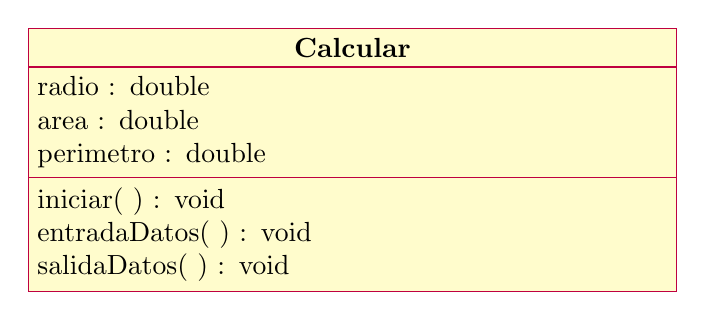
\begin{tikzpicture}
  \begin{class}[text width=8cm]{Calcular}{0,0}
    %\attribute{N : unsigned int}
    \attribute{radio : double}
    \attribute{area : double}
    \attribute{perimetro : double}    
    \operation{iniciar( ) : void}
    \operation{entradaDatos( ) : void}
    \operation{salidaDatos( ) : void}
    % virtual operations
    %\operation[0]{name(parameters list) : type of value returned}
    %\operation[0]{calcularArea() : void}
  \end{class}
\end{tikzpicture}
\end{center}

\end{document}